\chapter{Laboratorio 15/11/22}
In questa esperienza di laboratorio, si è presentata la board Arduino Nano 33 BLE Sense, una piattaforma open-source che integra diversi sensori e ne facilita l'utilizzo. In particolare, la piattaforma è dotata dei seguenti sensori (\Fig\ref{fig:arduino}):
\begin{itemize}
	\item LSM9DS1, una \textit{insertial measurement unit} (IMU) a 9 assi che integra un accelerometro, un giroscopio e un magnetometro;+
	\item LPS22HB che integra un barometro e un sensore di temperatura;
	\item HTS221, un sensore di umidità relativa;
	\item APDS-9960 che può essere usato come sensore di prossimità, luce ambientale, sensore RBG e movimenti;
	\item MP34DT05, un microfono digitale.
\end{itemize}
\begin{figure}[b!]
	\centering
	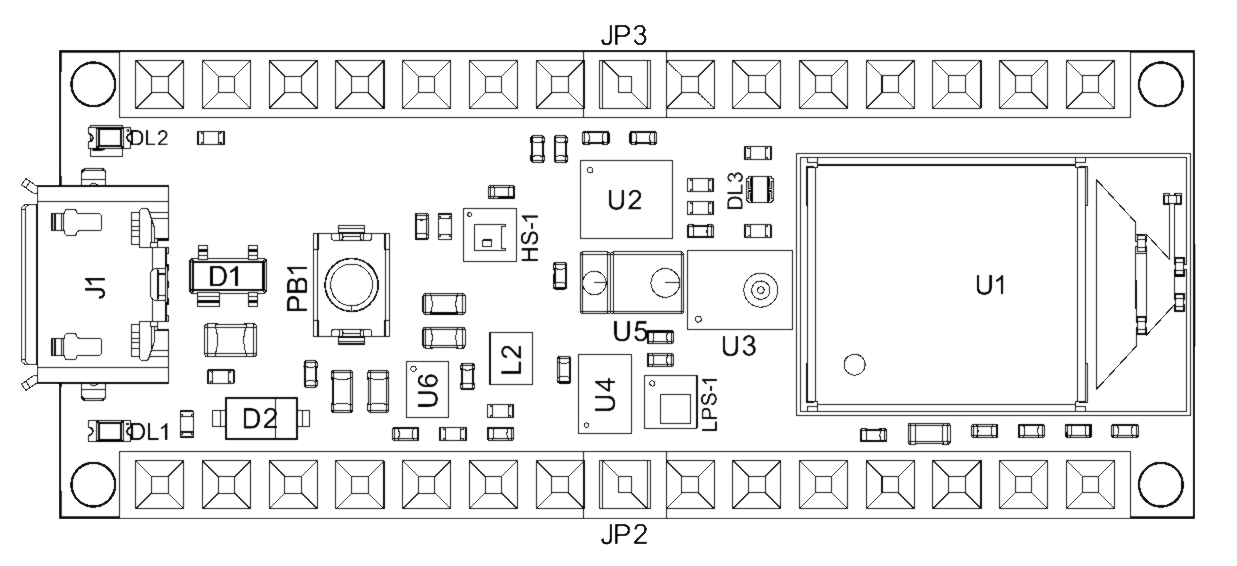
\includegraphics[width=0.8\linewidth]{./ImageFiles/arduino.png}
	\caption{Arduino Nano 33 BLE Sense, vista top. U1:NINA-B306 Module Bluetooth® Low Energy 5.0 Module, U2:LSM9DS1TR Sensor IMU, U3:MP34DT06JTR Mems Microphone, U4:ATECC608A Crypto chip, U5:APDS-9660 Ambient Module, U6:MP2322GQH Step Down Converter, PB1:IT-1185AP1C-160G-GTR Push button, HS-1:HTS221 Humidity Sensor, DL1:Led L, DL2: Led Power.}
	\label{fig:arduino}
\end{figure}
Inoltre, è presente un chip per la crittografia ATECC608A e un convertitore DC-DC MPM3610. Il microprocessore è integrato nel modulo NINA B306 (\SI{64}{\mega\hertz} Arm Cortex-M4F) che fornisce anche un modulo Bluetooth 5, con supporto multiprotocollo. La board viene alimentata con una tensione di \SI{3.3}{\volt}. Tipicamente l'alimentazione è fornita tramite la porta USB che viene anche utilizzata per il caricamento del firmware tramite l'Arduino IDE.